\bta{力学综合题(下)}
\begin{enumerate}
\renewcommand{\labelenumi}{\arabic{enumi}.}
% A(\Alph) a(\alph) I(\Roman) i(\roman) 1(\arabic)
%设定全局标号series=example	%引用全局变量resume=example
%[topsep=-0.3em,parsep=-0.3em,itemsep=-0.3em,partopsep=-0.3em]
%可使用leftmargin调整列表环境左边的空白长度 [leftmargin=0em]
\item
\exwhere{$ 2019 $年全国\lmd{1}卷}
竖直面内一倾斜轨道与一足够长的水平轨道通过一小段光滑圆弧平滑连
接,小物块$ B $静止于水平轨道的最左端,如图($ a $)所示。$ t=0 $时刻,小物块$ A $在倾斜轨道上从静止
开始下滑,一段时间后与$ B $发生弹性碰撞(碰撞时间极短);当$ A $返回到倾斜轨道上的$ P $点(图中未
标出)时,速度减为$ 0 $,此时对其施加一外力,使其在倾斜轨道上保持静止。物块$ A $运动的$ v-t $图像
如图($ b $)所示,图中的$ v_{1} $和$ t_{1} $均为未知量。已知$ A $的质量为$ m $,初始时$ A $与$ B $的高度差为$ H $,重力加
速度大小为$ g $,不计空气阻力。
\begin{enumerate}
\renewcommand{\labelenumi}{\arabic{enumi}.}
% A(\Alph) a(\alph) I(\Roman) i(\roman) 1(\arabic)
%设定全局标号series=example	%引用全局变量resume=example
%[topsep=-0.3em,parsep=-0.3em,itemsep=-0.3em,partopsep=-0.3em]
%可使用leftmargin调整列表环境左边的空白长度 [leftmargin=0em]
\item
求物块$ B $的质量;
\item 
在图($ b $)所描述的整个运动过程中,求物块 $ A $ 克服摩擦力所做的功;
\item 
已知两物块与轨道间的动摩擦因数均相等,在物块 $ B $ 停止运动后,改变物块与轨道间的动摩
擦因数,然后将 $ A $ 从 $ P $ 点释放,一段时间后 $ A $ 刚好能与 $ B $ 再次碰上。求改变前面动摩擦因数的比
值。



\end{enumerate}
\begin{figure}[h!]
\flushright
\includesvg[width=0.6\linewidth]{picture/svg/GZ-3-tiyou-0401}
\end{figure}




\banswer{
\begin{enumerate}
\renewcommand{\labelenumi}{\arabic{enumi}.}
% A(\Alph) a(\alph) I(\Roman) i(\roman) 1(\arabic)
%设定全局标号series=example	%引用全局变量resume=example
%[topsep=-0.3em,parsep=-0.3em,itemsep=-0.3em,partopsep=-0.3em]
%可使用leftmargin调整列表环境左边的空白长度 [leftmargin=0em]
\item
$3 m$
\item 
 $\frac{2}{15}mgH$ 
\item 
$\frac{11}{9}$



\end{enumerate}


}



\newpage
\item
\exwhere{$ 2018 $ 年全国\lmd{1}卷}
如图,$ abc $ 是竖直面内的光滑固定轨道,$ ab $ 水平,长度为 $ 2R $;$ bc $ 是半径为
$ R $ 的四分之一圆弧,与 $ ab $ 相切于 $ b $ 点。一质量为 $ m $ 的小球,始终受到与重力大小相等的水平外力
的作用,自 $ a $ 点处从静止开始向右运动。重力加速度大小为 $ g $。小球从
$ a $ 点开始运动到其轨迹最高点,机械能的增量为 \xzanswer{C} 
\begin{figure}[h!]
\centering
\includesvg[width=0.23\linewidth]{picture/svg/GZ-3-tiyou-0402}
\end{figure}


\fourchoices
{$ 2 mgR $}
{$ 4 mgR $}
{$ 5 mgR $}
{$ 6 mgR $}

\item 
\exwhere{$ 2018 $ 年天津卷}
滑雪运动深受人民群众的喜爱,某滑雪运动员(可视为质点)由坡道进入竖直
面内的圆弧形滑道 $ AB $,从滑道的 $ A $ 点滑行到最低点 $ B $ 的过程中,由于摩擦力的存在,运动员的速
率不变,则运动员沿 $ AB $ 下滑过程中 \xzanswer{C} 
\begin{figure}[h!]
\centering
\includesvg[width=0.23\linewidth]{picture/svg/GZ-3-tiyou-0403}
\end{figure}

\fourchoices
{所受合外力始终为零}
{所受摩擦力大小不变}
{合外力做功一定为零}
{机械能始终保持不变}



\item
\exwhere{$ 2018 $ 年全国\lmd{3}卷}
如图,在竖直平面内,一半径为 $ R $ 的光滑圆弧轨道 $ ABC $ 和水平
轨道 $ P_{A} $ 在 $ A $ 点相切,$ BC $ 为圆弧轨道的直径,$ O $ 为圆心,$ OA $ 和 $ OB $ 之间的夹角为 $ \alpha $, $ \sin \alpha = \frac{ 3 }{ 5 } $。
一质量为 $ m $ 的小球沿水平轨道向右运动,经 $ A $ 点沿圆弧轨道通过 $ C $ 点,落至水平轨道;在整个过
程中,除受到重力及轨道作用力外,小球还一直受到一水平
恒力的作用。已知小球在 $ C $ 点所受合力的方向指向圆心,
且此时小球对轨道的压力恰好为零。重力加速度大小为 $ g $。
求:
\begin{enumerate}
\renewcommand{\labelenumi}{\arabic{enumi}.}
% A(\Alph) a(\alph) I(\Roman) i(\roman) 1(\arabic)
%设定全局标号series=example	%引用全局变量resume=example
%[topsep=-0.3em,parsep=-0.3em,itemsep=-0.3em,partopsep=-0.3em]
%可使用leftmargin调整列表环境左边的空白长度 [leftmargin=0em]
\item
水平恒力的大小和小球到达 $ C $ 点时速度的大小;
\item 
小球到达 $ A $ 点时动量的大小;
\item 
小球从 $ C $ 点落至水平轨道所用的时间。




\end{enumerate}
\begin{figure}[h!]
\flushright
\includesvg[width=0.35\linewidth]{picture/svg/GZ-3-tiyou-0404}
\end{figure}

\banswer{
\begin{enumerate}
\renewcommand{\labelenumi}{\arabic{enumi}.}
% A(\Alph) a(\alph) I(\Roman) i(\roman) 1(\arabic)
%设定全局标号series=example	%引用全局变量resume=example
%[topsep=-0.3em,parsep=-0.3em,itemsep=-0.3em,partopsep=-0.3em]
%可使用leftmargin调整列表环境左边的空白长度 [leftmargin=0em]
\item
$v=\frac{\sqrt{5 g R}}{2}$
\item 
$p=m v_{1}=\frac{m \sqrt{23 g R}}{2}$
\item 
$t=\frac{3}{5} \sqrt{\frac{5 R}{g}}$
\end{enumerate}


}



\newpage
\item 
\exwhere{$ 2018 $年浙江卷($ 4 $月选考)}
如图所示,一轨道由半径为$ 2 \ m $的四分之一竖直圆弧轨道$ AB $和长
度可以调节的水平直轨道$ BC $在$ B $点平滑连接而成。现有一质量为$ 0.2 \ kg $的小球从$ A $点无初速度释放,
经过圆弧上的$ B $点时,传感器测得轨道所受压
力大小为$ 3.6 \ N $,小球经过$ BC $段所受阻力为其重
力的$ 0.2 $倍,然后从$ C $点水平飞离轨道,落到水
平面上的$ P $点,$ P $、$ C $两点间的高度差为$ 3.2 \ m $。小球运动过程中可以视为质点,且不计空气阻力。
\begin{enumerate}
\renewcommand{\labelenumi}{\arabic{enumi}.}
% A(\Alph) a(\alph) I(\Roman) i(\roman) 1(\arabic)
%设定全局标号series=example	%引用全局变量resume=example
%[topsep=-0.3em,parsep=-0.3em,itemsep=-0.3em,partopsep=-0.3em]
%可使用leftmargin调整列表环境左边的空白长度 [leftmargin=0em]
\item
求小球运动至$ B $点的速度大小;
\item 
求小球在圆弧轨道上克服摩擦力所做的功;
\item 
为使小球落点$ P $与$ B $点的水平距离最大,求$ BC $段的长度;
\item 
小球落到$ P $点后弹起,与地面多次碰撞后静止。假设小球每次碰撞机械能损失$ 75 \% $,碰撞前后
速度方向与地面的夹角相等。求小球从$ C $点飞出后静止所需的时间。



\end{enumerate}
\begin{figure}[h!]
\flushright
\includesvg[width=0.5\linewidth]{picture/svg/GZ-3-tiyou-0405}
\end{figure}

\banswer{
\begin{enumerate}
\renewcommand{\labelenumi}{\arabic{enumi}.}
% A(\Alph) a(\alph) I(\Roman) i(\roman) 1(\arabic)
%设定全局标号series=example	%引用全局变量resume=example
%[topsep=-0.3em,parsep=-0.3em,itemsep=-0.3em,partopsep=-0.3em]
%可使用leftmargin调整列表环境左边的空白长度 [leftmargin=0em]
\item
$v_{B}=4 \mathrm{m} / \mathrm{s}$
\item 
$W_{f}=2.4 \mathrm{J}$
\item 
$L_{B C}=3.36 \mathrm{m}$
\item 
$t=2.4 \mathrm{s}$
\end{enumerate}


}


\newpage

\item
\exwhere{$ 2011 $ 年理综山东卷}
如图所示,在高出水平地面 $ h=1.8 \ m $ 的光滑平台上放置一质量 $ M=2 \ kg $、由两种不同材料
连接成一体的薄板 $ A $,其右段长度 $ l_{1} =0.2 \ m $ 且表面光滑,左段表面粗糙。在 $ A $ 最右端放有可视为质点
的物块 $ B $,其质量 $ m=1 \ kg $。$ B $ 与 $ A $ 左段间动摩擦因数$ \mu =0.4 $。开始时二者均静止,现对 $ A $ 施加 $ F=20 \ N $
水平向右的恒力,待 $ B $ 脱离 $ A $($ A $ 尚未露出平台)后,将
A. 取走。$ B $ 离开平台后的落地点与平台右边缘的水平距离
$ x=1.2 \ m $。(取 $ g=10 \ m/s^{2} $)求:
\begin{enumerate}
\renewcommand{\labelenumi}{\arabic{enumi}.}
% A(\Alph) a(\alph) I(\Roman) i(\roman) 1(\arabic)
%设定全局标号series=example	%引用全局变量resume=example
%[topsep=-0.3em,parsep=-0.3em,itemsep=-0.3em,partopsep=-0.3em]
%可使用leftmargin调整列表环境左边的空白长度 [leftmargin=0em]
\item
$ B $ 离开平台时的速度 $ v_{B} $。
\item 
$ B $ 从开始运动到刚脱离 $ A $ 时,$ B $ 运动的时间 $ t_{B} $ 和位移 $ x_{B} $.

\item 
$ A $ 左端的长度 $ l_{2} $。




\end{enumerate}
\begin{figure}[h!]
\flushright
\includesvg[width=0.45\linewidth]{picture/svg/GZ-3-tiyou-0406}
\end{figure}


\banswer{
\begin{enumerate}
\renewcommand{\labelenumi}{\arabic{enumi}.}
% A(\Alph) a(\alph) I(\Roman) i(\roman) 1(\arabic)
%设定全局标号series=example	%引用全局变量resume=example
%[topsep=-0.3em,parsep=-0.3em,itemsep=-0.3em,partopsep=-0.3em]
%可使用leftmargin调整列表环境左边的空白长度 [leftmargin=0em]
\item
$v_{B}=2 \mathrm{m} / \mathrm{s}$
\item 
$t_{B}=0.5 \mathrm{s}$
 \qquad 
$x_{B}=0.5 \mathrm{m}$
\item 
$l_{2}=1.5 \mathrm{m}$
\end{enumerate}


}


\newpage
\item 
\exwhere{$ 2011 $ 年理综天津卷}
如图所示,圆管构成的半圆形轨道竖直固定在水平
地面上,轨道半径为 $ R $,$ MN $ 为直径且与水平面垂直,直径略小
于圆管内径的小球 $ A $ 以某一速度冲进轨道,到达半圆轨道最高点
$ M $ 时与静止于该处的质量与 $ A $ 相同的小球 $ B $ 发生碰撞,碰后两
球粘在一起飞出轨道,落地点距 $ N $ 为 $ 2R $。重力加速度为 $ g $,忽
略圆管内径,空气阻力及各处摩擦均不计,求:
\begin{enumerate}
\renewcommand{\labelenumi}{\arabic{enumi}.}
% A(\Alph) a(\alph) I(\Roman) i(\roman) 1(\arabic)
%设定全局标号series=example	%引用全局变量resume=example
%[topsep=-0.3em,parsep=-0.3em,itemsep=-0.3em,partopsep=-0.3em]
%可使用leftmargin调整列表环境左边的空白长度 [leftmargin=0em]
\item
粘合后的两球从飞出轨道到落地的时间 $ t $;
\item 
小球 $ A $ 冲进轨道时速度 $ v $ 的大小。




\end{enumerate}
\begin{figure}[h!]
\flushright
\includesvg[width=0.39\linewidth]{picture/svg/GZ-3-tiyou-0407}
\end{figure}


\banswer{
\begin{enumerate}
\renewcommand{\labelenumi}{\arabic{enumi}.}
% A(\Alph) a(\alph) I(\Roman) i(\roman) 1(\arabic)
%设定全局标号series=example	%引用全局变量resume=example
%[topsep=-0.3em,parsep=-0.3em,itemsep=-0.3em,partopsep=-0.3em]
%可使用leftmargin调整列表环境左边的空白长度 [leftmargin=0em]
\item
$t=2 \sqrt{\frac{R}{g}}$
\item 
$v_{2}=2 \sqrt{2 g R}$

\end{enumerate}


}


\newpage
\item 
\exwhere{$ 2011 $ 年物理江苏卷}
如图所示,长为 $ L $、内壁光滑的直管与水
平地面成 $ 30 ^{ \circ } $角固定放置。将一质量为 $ m $ 的小球固定在
管底,用一轻质光滑细线将小球与质量为 $ M=km $ 的小物
块相连,小物块悬挂于管口。现将小球释放,一段时间
后,小物块落地静止不动,小球继续向上运动,通过管
口的转向装置后做平抛运动,小球在转向过程中速率不
变。(重力加速度为 $ g $)
\begin{enumerate}
\renewcommand{\labelenumi}{\arabic{enumi}.}
% A(\Alph) a(\alph) I(\Roman) i(\roman) 1(\arabic)
%设定全局标号series=example	%引用全局变量resume=example
%[topsep=-0.3em,parsep=-0.3em,itemsep=-0.3em,partopsep=-0.3em]
%可使用leftmargin调整列表环境左边的空白长度 [leftmargin=0em]
\item
求小物块下落过程中的加速度大小;
\item 
求小球从管口抛出时的速度大小;
\item 
试证明小球平抛运动的水平位移总小于$\frac{\sqrt{2}}{2} L$。




\end{enumerate}
\begin{figure}[h!]
\flushright
\includesvg[width=0.4\linewidth]{picture/svg/GZ-3-tiyou-0408}
\end{figure}


\banswer{
\begin{enumerate}
\renewcommand{\labelenumi}{\arabic{enumi}.}
% A(\Alph) a(\alph) I(\Roman) i(\roman) 1(\arabic)
%设定全局标号series=example	%引用全局变量resume=example
%[topsep=-0.3em,parsep=-0.3em,itemsep=-0.3em,partopsep=-0.3em]
%可使用leftmargin调整列表环境左边的空白长度 [leftmargin=0em]
\item
$\frac{2 k-1}{2(k+1)} g$
\item 
$\sqrt{\frac{k-2}{2(k+1)} g L}(k>2) $ 
\item 
略



\end{enumerate}


}


\newpage
\item 
\exwhere{$ 2014 $ 年物理江苏卷}
如图所示,生产车间有两个相互垂直且等高的水平传送带甲和乙,甲的速度为 $ v_{0} $,小工
件离开甲前与甲的速度相同,并平稳地传到乙上,工件与乙之间的动摩擦因数为 $ \mu $. 乙的宽度足够
大,重力加速度为 $ g $.
\begin{enumerate}
\renewcommand{\labelenumi}{\arabic{enumi}.}
% A(\Alph) a(\alph) I(\Roman) i(\roman) 1(\arabic)
%设定全局标号series=example	%引用全局变量resume=example
%[topsep=-0.3em,parsep=-0.3em,itemsep=-0.3em,partopsep=-0.3em]
%可使用leftmargin调整列表环境左边的空白长度 [leftmargin=0em]
\item
若乙的速度为 $ v_{0} $,求工件在乙上侧向( 垂直于乙的运动
传送带甲
方向)滑过的距离 $ s $;


\item 
若乙的速度为 $ 2 v_{0} $,求工件在乙上刚停止侧向滑动时的
速度大小 $ v $



\item 
保持乙的速度 $ 2 v_{0} $ 不变,当工件在乙上刚停止滑动时,
下一只工件恰好传到乙上,如此反复. 若每个工件的质量均为 $ m $,除工件与传送带之间摩擦外,其
他能量损耗均不计,求驱动乙的电动机的平均输出功率 $ \bar{P} $.




\end{enumerate}
\begin{figure}[h!]
\flushright
\includesvg[width=0.4\linewidth]{picture/svg/GZ-3-tiyou-0409}
\end{figure}


\banswer{
\begin{enumerate}
\renewcommand{\labelenumi}{\arabic{enumi}.}
% A(\Alph) a(\alph) I(\Roman) i(\roman) 1(\arabic)
%设定全局标号series=example	%引用全局变量resume=example
%[topsep=-0.3em,parsep=-0.3em,itemsep=-0.3em,partopsep=-0.3em]
%可使用leftmargin调整列表环境左边的空白长度 [leftmargin=0em]
\item
$\frac{\sqrt{2} v_{0}^{2}}{2 \mu g}$
\item 
$2 v_{0}$
\item 
$\frac{4 \sqrt{5}}{5} \mu m g v_{0}$



\end{enumerate}


}





\newpage
\item
\exwhere{$ 2014 $ 年理综安徽卷}
在光滑水平地面上有一凹槽 $ A $,中央放一小物块 $ B $。物块与左右两边槽壁的距离如图
所示,$ L $ 为 $ 1.0 \ m $。凹槽与物块的质量均为 $ m $,两者之间的动摩擦因数$ \mu $为 $ 0.5 $。开始时物块静止,
凹槽以 $ v_{0} =5 \ m/s $ 初速度向右运动,设物块与凹槽壁碰撞过程中没有能量损失,且碰撞时间不计。$ g $
取 $ 10 \ m/s^{2} $。求:
\begin{enumerate}
\renewcommand{\labelenumi}{\arabic{enumi}.}
% A(\Alph) a(\alph) I(\Roman) i(\roman) 1(\arabic)
%设定全局标号series=example	%引用全局变量resume=example
%[topsep=-0.3em,parsep=-0.3em,itemsep=-0.3em,partopsep=-0.3em]
%可使用leftmargin调整列表环境左边的空白长度 [leftmargin=0em]
\item
物块与凹槽相对静止时的共同速度;

\item 
从凹槽开始运动到两者相对静止物块与右侧槽壁
碰撞的次数;
\item 
从凹槽开始运动到两者相对静止所经历的时间及该时间内凹槽运动的位移大小。



\end{enumerate}
\begin{figure}[h!]
\flushright
\includesvg[width=0.45\linewidth]{picture/svg/GZ-3-tiyou-0410}
\end{figure}


\banswer{
\begin{enumerate}
\renewcommand{\labelenumi}{\arabic{enumi}.}
% A(\Alph) a(\alph) I(\Roman) i(\roman) 1(\arabic)
%设定全局标号series=example	%引用全局变量resume=example
%[topsep=-0.3em,parsep=-0.3em,itemsep=-0.3em,partopsep=-0.3em]
%可使用leftmargin调整列表环境左边的空白长度 [leftmargin=0em]
\item
$2.5 \mathrm{m} / \mathrm{s}$
\item 
$12.75 \mathrm{m}$
\item 
$ 6 $



\end{enumerate}


}


\newpage
\item 
\exwhere{$ 2014 $ 年理综四川卷}
石墨烯是近些年发现的一种新材料,其超高强度及超强导电、导热等非凡的物理化学性质有望使
21. 世纪的世界发生革命性的变化,其发现者由此获得 $ 2010 $ 年诺贝尔物理学奖。用石墨烯制作超
级缆绳,人类搭建“太空电梯”的梦想有望在本世纪实现。科学家们设想,通过地球同步轨道站向
地面垂下一条缆绳至赤道基站,电梯仓沿着这条缆绳运行,实现外太
空和地球之间便捷的物资交换。
\begin{enumerate}
\renewcommand{\labelenumi}{\arabic{enumi}.}
% A(\Alph) a(\alph) I(\Roman) i(\roman) 1(\arabic)
%设定全局标号series=example	%引用全局变量resume=example
%[topsep=-0.3em,parsep=-0.3em,itemsep=-0.3em,partopsep=-0.3em]
%可使用leftmargin调整列表环境左边的空白长度 [leftmargin=0em]
\item
若”太空电梯”将货物从赤道基站运到距地面高度为 $ h_{1} $ 的同步轨
道站,求轨道站内质量为 $ m_{1} $ 的货物相对地心运动的动能。设地球自
转角速度为$ \omega $,地球半径为 $ R $。
\item 
当电梯仓停在距地面高度 $ h_{2} =4R $ 的站点时,求仓内质量 $ m_{2} = 50 \ kg $ 的人对水平地板的压力大小。取地面附近重力加速度 $ g= 10 \ m/s^{2} $,地球自转角速度$ \omega =7.3 \times 10-5r_{a}d/s $,地球半径 $ R= 6.4 \times 10^{3} \ km $。




\end{enumerate}
% TODO: \usepackage{graphicx} required
\begin{figure}[h!]
\flushright 
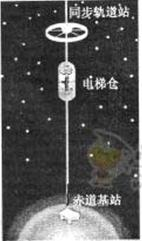
\includegraphics[width=0.15\linewidth]{picture/screenshot029}
\end{figure}


\banswer{
\begin{enumerate}
\renewcommand{\labelenumi}{\arabic{enumi}.}
% A(\Alph) a(\alph) I(\Roman) i(\roman) 1(\arabic)
%设定全局标号series=example	%引用全局变量resume=example
%[topsep=-0.3em,parsep=-0.3em,itemsep=-0.3em,partopsep=-0.3em]
%可使用leftmargin调整列表环境左边的空白长度 [leftmargin=0em]
\item
$E_{k}=\frac{1}{2} m_{1} \omega^{2}\left(R+h_{1}\right)^{2}$
\item 
$N^{\prime}=11.5 \mathrm{N}$

\end{enumerate}


}



\newpage
\item 
\exwhere{$ 2015 $ 年理综新课标 \lmd{1} 卷}
一长木板置于粗糙水平地面上,木板左端放置一小物块,在木
板右方有一墙壁,木板右端与墙壁的距离为 $ 4.5 \ m $,如图$ (a) $所示。$ t=0 $ 时刻开始,小物块与木板一起
以共同速度向右运动,直至 $ t=1 \ s $ 时
木板与墙壁碰撞(碰撞时间极短)。
碰撞前后木板速度大小不变,方向
相反;运动过程中小物块始终未离
开木板。已知碰撞后 $ 1 \ s $ 时间内小物
块的 $ v-t $ 图线如图$ (b) $所示。木板的
质量是小物块质量的 $ 15 $ 倍,重力加速度大小 $ g $ 取 $ 10 \ m/s $。求:
\begin{enumerate}
\renewcommand{\labelenumi}{\arabic{enumi}.}
% A(\Alph) a(\alph) I(\Roman) i(\roman) 1(\arabic)
%设定全局标号series=example	%引用全局变量resume=example
%[topsep=-0.3em,parsep=-0.3em,itemsep=-0.3em,partopsep=-0.3em]
%可使用leftmargin调整列表环境左边的空白长度 [leftmargin=0em]
\item
木板与地面间的动摩擦因数$ \mu _{1} $ 及小物块与木板间的动摩擦因数$ \mu _{2} $;



\item 
木板的最小长度;



\item 
木板右端离墙壁的最终距离。



\end{enumerate}
\begin{figure}[h!]
\flushright
\includesvg[width=0.55\linewidth]{picture/svg/GZ-3-tiyou-0411}
\end{figure}

\banswer{
\begin{enumerate}
\renewcommand{\labelenumi}{\arabic{enumi}.}
% A(\Alph) a(\alph) I(\Roman) i(\roman) 1(\arabic)
%设定全局标号series=example	%引用全局变量resume=example
%[topsep=-0.3em,parsep=-0.3em,itemsep=-0.3em,partopsep=-0.3em]
%可使用leftmargin调整列表环境左边的空白长度 [leftmargin=0em]
\item
$\mu_{2}=0.4$

\item 
木板的最小长度应为6.0 m。

\item 
最终距离为6.5 m。

\end{enumerate}


}


\newpage
\item 
\exwhere{$ 2015 $ 年理综新课标$ \lmd{2} $卷}
下暴雨时,有时会发生山体滑坡或泥石流等地质灾害。某
地有一倾角为$ \theta =37 ^{ \circ } ( \sin 37 ^{ \circ } = \frac{ 3 }{ 5 } ) $
的山坡 $ C $,上面有一质量为 $ m $ 的石板 $ B $,其上下表面与斜坡平
行;$ B $ 上有一碎石堆 $ A $(含有大量泥土)
,$ A $ 和 $ B $ 均处于静止状态,如图所示。假设某次暴雨中,$ A $
浸透雨水后总质量也为 $ m $(可视为质量不变的滑块),在极短时间内,$ A $、$ B $ 间的动摩擦因数$ \mu _{1} $ 减小
为
$ \frac{ 3 }{ 8 } $
,$ B $、$ C $ 间的动摩擦因数$ \mu _{2} $ 减小为 $ 0.5 $,$ A $、$ B $ 开始运动,此时
刻为计时起点;在第 $ 2 \ s $ 末,$ B $ 的上表面突然变为光滑,$ \mu _{2} $ 保持不
变。已知 $ A $ 开始运动时,$ A $ 离 $ B $ 下边缘的距离 $ l=27 \ m $,$ C $ 足够长,
设最大静摩擦力等于滑动摩擦力。取重力加速度大小 $ g=10 \ m/s^{2} $。
求:
\begin{enumerate}
\renewcommand{\labelenumi}{\arabic{enumi}.}
% A(\Alph) a(\alph) I(\Roman) i(\roman) 1(\arabic)
%设定全局标号series=example	%引用全局变量resume=example
%[topsep=-0.3em,parsep=-0.3em,itemsep=-0.3em,partopsep=-0.3em]
%可使用leftmargin调整列表环境左边的空白长度 [leftmargin=0em]
\item
在 $ 0 \sim 2 \ s $ 时间内 $ A $ 和 $ B $ 加速度的大小;

\item 
$ A $ 在 $ B $ 上总的运动时间。



\end{enumerate}
\begin{figure}[h!]
\flushright
\includesvg[width=0.25\linewidth]{picture/svg/GZ-3-tiyou-0412}
\end{figure}


\banswer{
\begin{enumerate}
\renewcommand{\labelenumi}{\arabic{enumi}.}
% A(\Alph) a(\alph) I(\Roman) i(\roman) 1(\arabic)
%设定全局标号series=example	%引用全局变量resume=example
%[topsep=-0.3em,parsep=-0.3em,itemsep=-0.3em,partopsep=-0.3em]
%可使用leftmargin调整列表环境左边的空白长度 [leftmargin=0em]
\item
$a_{1}=3 \mathrm{m} / \mathrm{s}^{2}$ \qquad 
$a_{2}=1 \mathrm{m} / \mathrm{s}^{2}$

\item 
$t_{\text {总 }}=t_{1}+t_{2}+t_{3}=4 \ \mathrm{s}$
\end{enumerate}


}


\newpage
\item 
\exwhere{$ 2015 $ 年理综福建卷}
如图,质量为 $ M $ 的小车静止在光滑水平面上,小车 $ AB $ 段是半
径为 $ R $ 的四分之一圆弧光滑轨道,$ BC $ 段是长为 $ L $ 的水平粗糙轨道,两段轨道相切于 $ B $ 点。一质量
为 $ m $ 的滑块在小车上从 $ A $ 点由静止开始沿轨道滑下,重力加速度为 $ g $。
\begin{enumerate}
\renewcommand{\labelenumi}{\arabic{enumi}.}
% A(\Alph) a(\alph) I(\Roman) i(\roman) 1(\arabic)
%设定全局标号series=example	%引用全局变量resume=example
%[topsep=-0.3em,parsep=-0.3em,itemsep=-0.3em,partopsep=-0.3em]
%可使用leftmargin调整列表环境左边的空白长度 [leftmargin=0em]
\item
若固定小车,求滑块运动过程中对小车的最大压力;



\item 
若不固定小车,滑块仍从 $ A $ 点由静止下滑,然后滑入 $ BC $ 轨道,最后从
$ C $点滑出小车。已知滑块质量 $m=\frac{M}{2}$
,在任一时刻滑块相对地面速度的水
平分量是小车速度大小的 $ 2 $ 倍,滑块与轨道 $ BC $ 间的动摩擦因数为$ \mu $,求$ : $

①滑块运动过程中,小车的最大速度大小 $ v_{m} $;

②滑块从 $ B $ 到 $ C $ 运动过程中,小车的位移大小 $ s $。




\end{enumerate}
\begin{figure}[h!]
\flushright
\includesvg[width=0.25\linewidth]{picture/svg/GZ-3-tiyou-0413}
\end{figure}

\banswer{
\begin{enumerate}
\renewcommand{\labelenumi}{\arabic{enumi}.}
% A(\Alph) a(\alph) I(\Roman) i(\roman) 1(\arabic)
%设定全局标号series=example	%引用全局变量resume=example
%[topsep=-0.3em,parsep=-0.3em,itemsep=-0.3em,partopsep=-0.3em]
%可使用leftmargin调整列表环境左边的空白长度 [leftmargin=0em]
\item
$3 m g$
\item 
①$v_{m}=\sqrt{\frac{1}{3} g R}$ \qquad ②$s=L / 3$



\end{enumerate}


}


\newpage
\item 
\exwhere{$ 2015 $ 年江苏卷}
一转动装置如图所示,四根轻杆 $ OA $、$ OC $、$ AB $ 和 $ CB $ 与两小球及一小
环通过铰链连接,轻杆长均为 $ l $,球和环的质量均为 $ m $,$ O $ 端固定在竖直的轻质转轴上。 套在转轴
上的轻质弹簧连接在 $ O $ 与小环之间,原长为 $ L $. 装置静止时,弹簧长
为
$ \frac{ 2 }{ 3 } L $. 转动该装置并缓慢增大转速,小环缓慢上升。弹簧始终在弹
性限度内,忽略一切摩擦和空气阻力,重力加速度为 $ g $.
求:
\begin{enumerate}
\renewcommand{\labelenumi}{\arabic{enumi}.}
% A(\Alph) a(\alph) I(\Roman) i(\roman) 1(\arabic)
%设定全局标号series=example	%引用全局变量resume=example
%[topsep=-0.3em,parsep=-0.3em,itemsep=-0.3em,partopsep=-0.3em]
%可使用leftmargin调整列表环境左边的空白长度 [leftmargin=0em]
\item
弹簧的劲度系数 $ k $;



\item 
$ AB $ 杆中弹力为零时,装置转动的角速度 $ \omega_0 $;

\item 
弹簧长度从 $ \frac{ 3 }{ 2 } L $ 缓慢缩短为 $ \frac{ 1 }{ 2 } L $ 的过程中,外界对转动装置所做的功 $ W $.


\end{enumerate}
\begin{figure}[h!]
\flushright
\includesvg[width=0.25\linewidth]{picture/svg/GZ-3-tiyou-0414}
\end{figure}


\banswer{
\begin{enumerate}
\renewcommand{\labelenumi}{\arabic{enumi}.}
% A(\Alph) a(\alph) I(\Roman) i(\roman) 1(\arabic)
%设定全局标号series=example	%引用全局变量resume=example
%[topsep=-0.3em,parsep=-0.3em,itemsep=-0.3em,partopsep=-0.3em]
%可使用leftmargin调整列表环境左边的空白长度 [leftmargin=0em]
\item
$ k=\frac{4 m g}{L}$
\item 
 $\omega_{0}=\sqrt{\frac{8 g}{5 L}}$
\item 
 $W=m g L+\frac{16 m g l^{2}}{L}$



\end{enumerate}


}


\newpage
\item 
\exwhere{$ 2016 $ 年新课标$ \lmd{2} $卷}
轻质弹簧原长为 $ 2l $,将弹簧竖直放置在地面上,在其顶端将一
质量为 $ 5 \ m $ 的物体由静止释放,当弹簧被压缩到最短时,弹簧长度为 $ l $。现将该弹簧水平放置,一
端固定在 $ A $ 点,另一端与物块 $ P $ 接触但不连接。$ AB $ 是长度为 $ 5l $ 的水平轨道,$ B $ 端与半径为 $ l $ 的光
滑半圆轨道 $ BCD $ 相切,半圆的直径 $ BD $ 竖直,如图所示。物块 $ P $ 与 $ AB $ 间的动摩擦因数$ \mu =0.5 $。用
外力推动物块 $ P $,将弹簧压缩至长度 $ l $,然后放开,$ P $ 开始
沿轨道运动,重力加速度大小为 $ g $。
\begin{enumerate}
\renewcommand{\labelenumi}{\arabic{enumi}.}
% A(\Alph) a(\alph) I(\Roman) i(\roman) 1(\arabic)
%设定全局标号series=example	%引用全局变量resume=example
%[topsep=-0.3em,parsep=-0.3em,itemsep=-0.3em,partopsep=-0.3em]
%可使用leftmargin调整列表环境左边的空白长度 [leftmargin=0em]
\item
若 $ P $ 的质量为 $ m $,求 $ P $ 到达 $ B $ 点时速度的大小,以
及它离开圆轨道后落回到 $ AB $ 上的位置与 $ B $ 点间的距离;

\item 
若 $ P $ 能滑上圆轨道,且仍能沿圆轨道滑下,求 $ P $ 的
质量的取值范围。



\end{enumerate}
\begin{figure}[h!]
\flushright
\includesvg[width=0.4\linewidth]{picture/svg/GZ-3-tiyou-0415}
\end{figure}



\banswer{
\begin{enumerate}
\renewcommand{\labelenumi}{\arabic{enumi}.}
% A(\Alph) a(\alph) I(\Roman) i(\roman) 1(\arabic)
%设定全局标号series=example	%引用全局变量resume=example
%[topsep=-0.3em,parsep=-0.3em,itemsep=-0.3em,partopsep=-0.3em]
%可使用leftmargin调整列表环境左边的空白长度 [leftmargin=0em]
\item
$2 \sqrt{2 l}$
\item 
 $\frac{5}{3} m \leq M<\frac{5}{2} m$



\end{enumerate}


}



\newpage
\item 
\exwhere{$ 2016 $ 年新课标 \lmd{1} 卷}
如图,一轻弹簧原长为 $ 2R $,其一端固定在倾角为 $ 37 ^{ \circ } $的固定直轨道 $ AC $ 的底端 $ A $ 处,另一端位于直
轨道上 $ B $ 处,弹簧处于自然状态。直轨道与一半径为 $ \frac{ 5 }{ 6 } R $ 的光滑圆弧轨道相切于 $ C $ 点,$ AC=7R $,
$ A $、$ B $、$ C $、$ D $ 均在同一竖直平面内。质量为 $ m $ 的小物块 $ P $ 自 $ C $ 点由静止开始下滑,最低到达 $ E $ 点
(未画出)随后 $ P $ 沿轨道被弹回,最高到达 $ F $ 点,$ AF=4R $。已知 $ P $ 与直轨道间的动摩擦因数
$ \mu= \frac{ 1 }{ 4 } $,重力加速度大小为 $ g $。(取 $ \sin 37 ^{ \circ } = \frac{ 3 }{ 5 } $, $ \cos 37 ^{ \circ } = \frac{ 4 }{ 5 } $ )
\begin{enumerate}
\renewcommand{\labelenumi}{\arabic{enumi}.}
% A(\Alph) a(\alph) I(\Roman) i(\roman) 1(\arabic)
%设定全局标号series=example	%引用全局变量resume=example
%[topsep=-0.3em,parsep=-0.3em,itemsep=-0.3em,partopsep=-0.3em]
%可使用leftmargin调整列表环境左边的空白长度 [leftmargin=0em]
\item
求 $ P $ 第一次运动到 $ B $ 点时速度的大小。

\item 
求 $ P $ 运动到 $ E $ 点时弹簧的弹性势能。



\item 
改变物块 $ P $ 的质量,将 $ P $ 推至 $ E $ 点,从静止开始释放。已
知 $ P $ 自圆弧轨道的最高点 $ D $ 处水平飞出后,恰好通过 $ G $ 点。
$ G $ 点在 $ C $ 点的左下方,与 $ C $ 点水平相距 $ \frac{ 7 }{ 2 } R $、竖直相距 $ R $,
求 $ P $ 运动到 $ D $ 点时速度的大小和改变后 $ P $ 的质量。




\end{enumerate}
\begin{figure}[h!]
\flushright
\includesvg[width=0.35\linewidth]{picture/svg/GZ-3-tiyou-0416}
\end{figure}

\banswer{
\begin{enumerate}
\renewcommand{\labelenumi}{\arabic{enumi}.}
% A(\Alph) a(\alph) I(\Roman) i(\roman) 1(\arabic)
%设定全局标号series=example	%引用全局变量resume=example
%[topsep=-0.3em,parsep=-0.3em,itemsep=-0.3em,partopsep=-0.3em]
%可使用leftmargin调整列表环境左边的空白长度 [leftmargin=0em]
\item
$v_{B}=2 \sqrt{g R}$

\item 
$E_{\text {弹 }} \text{为} \frac{12 m g R}{5}$
\item 
$v_{0}=\frac{3 \sqrt{5 g R}}{5}$ \qquad $m^{\prime}=\frac{1}{3} m$
\end{enumerate}


}



\newpage
\item 
\exwhere{$ 2017 $ 年浙江选考卷}
图中给出一段“ $ S $ ”形单行盘山公路的示意图,弯道 $ 1 $、弯道 $ 2 $ 可看作两个
不同水平面上的圆弧,圆心分别为 $ O_{1},O_{2} $,弯道中心线半径分别为 $ r_{1} =10 \ m, r_{2} =20 \ m $,弯道 $ 2 $
比弯道 $ 1 $ 高 $ h=12 \ m $,有一直道与两弯道圆弧相切。质量 $ m=1200 \ kg $ 的汽车通过弯道时做匀速圆
周运动,路面对轮胎的最大径向静摩擦力是车重的 $ 1.25 $ 倍,行驶时要求汽车不打滑。
($ \sin 37 ^{ \circ } =0.6 $,$ \sin 53 ^{ \circ } =0.8 $)
\begin{enumerate}
\renewcommand{\labelenumi}{\arabic{enumi}.}
% A(\Alph) a(\alph) I(\Roman) i(\roman) 1(\arabic)
%设定全局标号series=example	%引用全局变量resume=example
%[topsep=-0.3em,parsep=-0.3em,itemsep=-0.3em,partopsep=-0.3em]
%可使用leftmargin调整列表环境左边的空白长度 [leftmargin=0em]
\item
求汽车沿弯道 $ 1 $ 中心线行驶时的最大速度 $ v_{1} $;

\item 
汽车以 $ v_{1} $ 进入直道,以 $ P=30 \ kW $ 的恒定功率直线行驶了
$ t=8.0 \ s $,进入弯道 $ 2 $,此时速度恰为通过弯道 $ 2 $ 中心线的最大速
度,求直道上除重力以外的阻力对汽车做的功;

\item 
汽车从弯道 $ 1 $ 的 $ A $ 点进入,从同一直径上的 $ B $ 点驶离,有经验的司机会利用路面宽度,用最
短时间匀速安全通过弯道,设路宽 $ d=10 \ m $,求此最短时间($ A $、$ B $ 两点都在轨道的中心线上,计
算时视汽车为质点 )。



\end{enumerate}
\begin{figure}[h!]
\flushright
\includesvg[width=0.4\linewidth]{picture/svg/GZ-3-tiyou-0417}
\end{figure}

\banswer{
\begin{enumerate}
\renewcommand{\labelenumi}{\arabic{enumi}.}
% A(\Alph) a(\alph) I(\Roman) i(\roman) 1(\arabic)
%设定全局标号series=example	%引用全局变量resume=example
%[topsep=-0.3em,parsep=-0.3em,itemsep=-0.3em,partopsep=-0.3em]
%可使用leftmargin调整列表环境左边的空白长度 [leftmargin=0em]
\item
$v_{1}=5 \sqrt{5} \mathrm{m} / \mathrm{s}$ 
\item 
$W_{f}=-2.1 \times 10^{4} \mathrm{J}$ 
\item 
$t^{\prime}=1.8 \ \mathrm{s}$



\end{enumerate}


}









\end{enumerate}

